\section{Grundlegendes Prinzip von LabVIEW}

Das Erstellen eines Programmes in LabVIEW findet über eine grafische Oberfläche statt, welche in zwei Bereiche aufgeteilt ist.
Das \textbf{Frontpanel} beinhaltet Steuerelemente zur Interaktion mit dem Nutzer des Programmes. Beispiel für solche Steuerelemente sind Schalter, Regler und Diagramme. Das \textbf{Blockdiagramm} beinhaltet Funktionsblöcke sowie Repräsentationen der auf dem Frontpanel befindlichen Steuerelemente, die mit Verbindungslinien verbunden werden, welche den Datenfluss steuern.
Die in LabVIEW erstellten Programme liegen in Form sogenannter VIs (virtual instruments) vor. Jedes Programm ist eigenständig lauffähig, kann aber auch als Unterprogramm in anderen VIs verwendet werden.

\subsection{Berechnung von Produkt und Fakultät}

Zur Verinnerlichung dieses Prinzips wurde ein Programm mit vergleichsweise einfachem Aufbau konstruiert, mit welchem das Produkt zweier Zahlen, und die Fakultät einer Zahl berechnet werden konnte. Das Blockdiagramm und das Frontpanel sind in Abbildung \ref{fig:fup} dargestellt.

\

\begin{figure}[ht]
	\centering
	\begin{subfigure}[c]{0.55\textwidth}
		\centering
		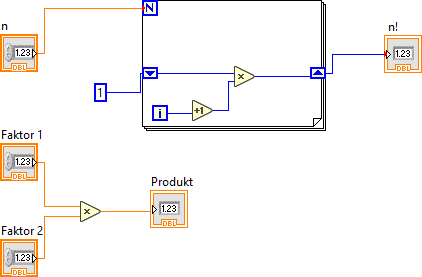
\includegraphics[width=\textwidth]{pic/fup1.png}
		\caption{Blockdiagramm}
	\end{subfigure}
	\begin{subfigure}[c]{0.35\textwidth}
		\centering
		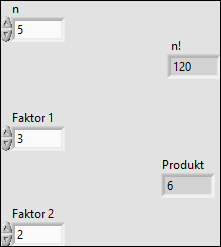
\includegraphics[width=\textwidth]{pic/fup2.png}
		\caption{Frontpanel}
	\end{subfigure}
	\caption{Diese Grafik zeigt das Blockdiagramm (links) und das Frontpanel (rechts) des besagten Programmes zur Berechnung von Produkten und Fakultäten. Es ist der Output des Programmes für drei beispielhafte Zahlen zu sehen.}
	\label{fig:fup}	
\end{figure}

\

Im unteren Teil des Blockdiagrammes (Abb. \ref{fig:fup} u.r.) ist der (grafische) Code zur Berechnung des Produkts zweier Zahlen enthalten. Die beiden Datenquellen (Variablen des Typs Double mit den Bezeichnungen Faktor 1 und Faktor 2) sind mit einem Funktionsblock verbunden, welcher die mathematische Operation der Multiplikation durchführt. Der Output des Funktionsblockes ist mit einem Indikator (Datensenke) verbunden. Die Datenquellen und -senken sind mit Bedien- und Anzeigeelementen auf dem Frontpanel verknüpft (Abb. \ref{fig:fup} u.l.).

Im oberen Teil des Blockdiagrammes (Abb. \ref{fig:fup} o.l.) ist der Code zur Berechnung der Fakultät der Variable n (Typ: Double) enthalten. Die Datenquelle ist mit einer for-Schleife (umrandetes Rechteck) verbunden und gibt die Zahl der Wiederholungen an. Die for-Schleife beinhaltet ein Schieberegister (Startwert: 1, bestimmt durch die Konstante links außerhalb der Schleife), das Inkrement (Startwert: 0), und einen Multiplikationsoperator.

In jedem Schleifendurchlauf wird das Inkrement mit dem aktuellen Inhalt des Schieberegisters multipliziert, und das Ergebnis der Multiplikation als neuer Wert des Registers übernommen. Um eine Multiplikation mit Null zu vermeiden wird das Inkrement durch den „+1“-Block zusätzlich um 1 erhöht. Der Inhalt des Schieberegisters wird nach Durchlauf der Schleife an eine Datensenke weitergereicht. Wie auch beim Programmteil zur Berechnung des Produktes sind Datenquelle und -senke mit entsprechenden Elementen auf dem Frontpanel verbunden.

\subsection{Programm zur Darstellung einer Sinusfunktion}

Nach Fertigstellung des VIs zur Berechnung von Produkt und Fakultät wurde ein Programm geschrieben, welches ein Array mit Funktionswerten einer Sinusfunktion füllte und grafisch ausgab. Genauer wurde eine Sinusfunktion des Typs $A\cdot \sin( \omega t + \Phi)$ realisiert, mit variabler Amplitude $A$, Winkelgeschwindigkeit $ \omega=2 \pi f$ und Phase $\Phi$. Blockdiagramm und Frontpanel des Programms sind in Abbildung \ref{fig:sinus} dargestellt.

\

Zur Berechnung der Zeitlichen Komponente $t$ der Funktion wurde eine for-Schleife verwendet (vgl. Abb. \ref{fig:sinusB} o.l.). Diese erhält als Input einen Wert $N$, und gibt in jeden Durchlauf den Wert $i/N$ aus, so dass die Zeitreihe $0/N$, $1/N$, …, $(N-1)/N$ entsteht. Diese wird als Definitionsmenge an das Array weitergereicht.

\begin{figure}[H]
	\centering
	\begin{subfigure}[c]{\textwidth}
		\centering
		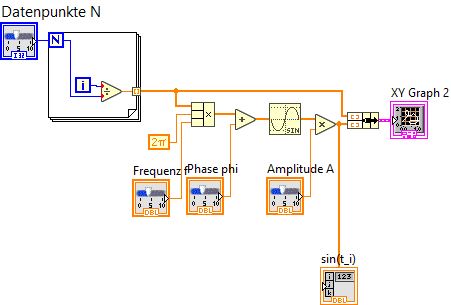
\includegraphics[width=0.6\textwidth]{pic/sinBlock.png}
		\caption{Blockdiagramm des Sinus-VI}
		\label{fig:sinusB}
	\end{subfigure}
	
	\
	
	\
	
	\begin{subfigure}[c]{\textwidth}
		\centering
		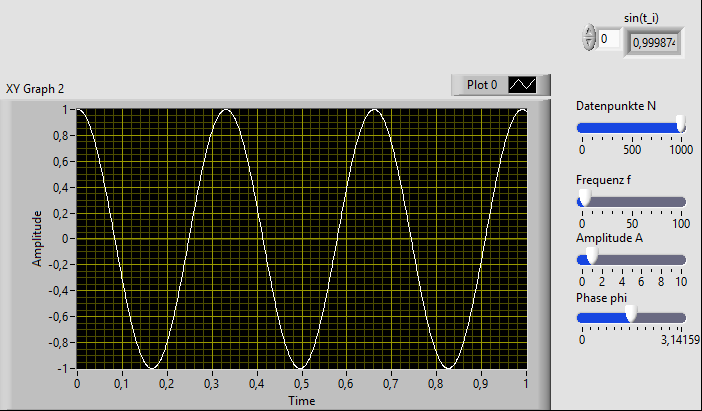
\includegraphics[width=\textwidth]{pic/sinFront.png}
		\caption{Frontpanel des Sinus-VI}
		\label{fig:sinusF}
	\end{subfigure}
	\caption{Diese Grafik zeigt das Blockdiagramm (oben) und das Frontpanel (unten) des Sinus-VIs. Es ist der Output des Programmes für einen um ca. $\pi / 2$ phasenverschobenen Sinus mit geringer Frequenz und Amplitude dargestellt.}
	\label{fig:sinus}	
\end{figure}

\

\

Zur Berechnung des Wertebereichs wird die mit der for-Schleife berechnete Zeitkomponente mit der Konstante $2 \pi$ und der variablen Frequenz $f$ multipliziert. Zu dem Produkt wird anschließend die variable Phase $\Phi$ addiert. Mittels einem von LabVIEW zur Verfügung gestellten Funktionsblock wird der Sinus der Summe berechnet, welcher anschließend mit der Amplitude $A$ multipliziert wird. Das gefüllte Array wird an den Funktionsblock „XY Graph 2“ weitergereicht, mit dessen Hilfe die Daten auf dem Frontpanel grafisch dargestellt werden. Um einzelne Werte des Arrays überprüfen zu können, wird der Wertebereich zusätzlich mit einem Indikator verbunden ("$\sin(t_i)$", vgl. Abb. \ref{fig:sinusB} unten).
Auf dem Frontpanel (vgl. Abb. \ref{fig:sinusF}) sind die mit den Variablen $N$, $f$, $\Phi$  und $A$ verknüpften Steuerelemente, der Graph und der Indikator zu sehen. 

\subsection{Programm zur Darstellung von Lissajous-Figuren}

Um die Funktion von VIs als Unterprogramme zu zeigen, wurde ein Programm erstellt, welches mit Hilfe des vorher erstellten Sinus-VI Lissajous-Figuren zeichnen kann. Als Lissajous-Figuren werden Überlagerungskurven zweier orthogonal aufeinander stehender harmonischer Schwingungen bezeichnet. Diese lassen sich mathematisch als Abbildungen folgender Form beschreiben:

\

\begin{equation}
 t \mapsto 	\begin{pmatrix}
		 A_x\sin(2\pi f_1 t + \phi_1) \\ 
		 A_y\sin(2\pi f_2 t + \phi_2)
	 \end{pmatrix},
	 \quad	t \in [0,\infty)
\end{equation}

\

Zum Zeichnen der Figuren wurde ein s.g. Express-VI verwendet, welches aus einem "X-Input" und einem "Y-Input" in dynamischem Format ohne weitere Einstellungen einen „XY Graph“ erstellt (vgl. Blockdiagramm, Abb. \ref{fig:LissajouBlock}). Für die beiden Inputs wurde jeweils das vorher erstellte Sinus-Programm verwendet. Letzteres wurde so eingestellt, dass es Amplitude, Frequenz und Phase als Input entgegennimmt, und das mit den Funktionswerten gefüllte Array ausgibt.

\

\begin{figure}[H]
	\centering
	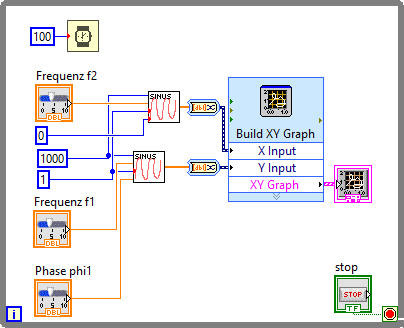
\includegraphics[width=0.6\textwidth]{pic/LisBlock.png}
	\caption{Diese Grafik stellt das Blockdiagramm der Lissajou-VI dar.}
	\label{fig:LissajouBlock}	
\end{figure} 

\

Das Express-VI samt In- und Output wurde in einer While-Schleife platziert, damit die Parameter während der Ausführung des Programmes geändert werden können, und die Änderungen direkt sichtbar werden. Man beachte den „stop“-Button (vgl. Abb. \ref{fig:LissajouBlock} u.r.), mit dem die Schleife unterbrochen wird, und die Clock (vgl. Abb. \ref{fig:LissajouBlock} o.r.), welche die Wartezeit zwischen zwei Schleifendurchläufen bestimmt. Letztere wurde auf einen Wert von \SI{100}{\milli\second} eingestellt, welcher gering genug ist um das Programm subjektiv flüssig darzustellen, aber hoch genug um die CPU-Auslastung merklich zu reduzieren.
Beispiele für zwei Lissajou-Figuren sind in Abb. \ref{fig:LissajouFront} zu sehen.
\

\begin{figure}[H]
	\centering
	\begin{subfigure}[c]{\textwidth}
		\centering
		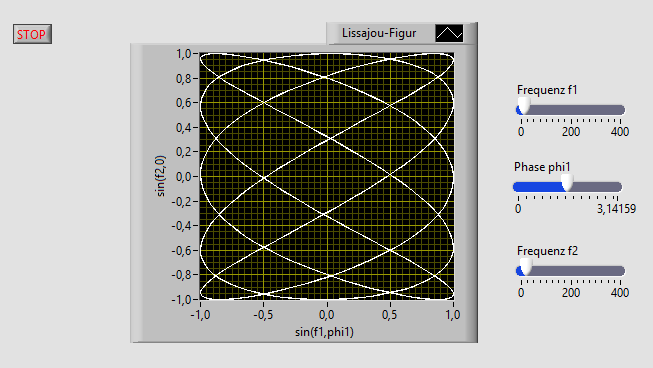
\includegraphics[width=\textwidth]{pic/LissFront1.png}
	\end{subfigure}
	\begin{subfigure}[c]{\textwidth}
		\centering
		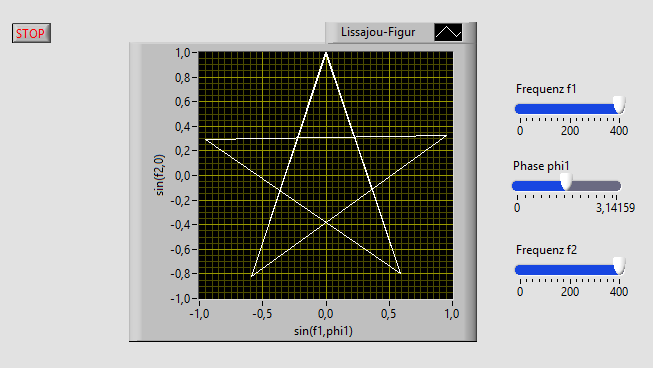
\includegraphics[width=\textwidth]{pic/LissFront2.png}
	\end{subfigure}
	\caption{Diese Grafik zeigt zwei Beispiele für Lissajou-Figuren auf dem Frontpanel der Lissajou-VI.}
	\label{fig:LissajouFront}	
\end{figure}